\subsection{Drivetrain}
The drivetrain of a motored vehicle, is the components that transfer the rotational energy from the motor to the driving wheel of the vehicle. For this vehicle, the drivetrain will contain the gear connected to the brushed DC motor, the differential gear box and the gears connected to the belts. The drivetrain is shown on \figref{vehicleDescriptionDriveTrain}.

\begin{figure}[H]
	\centering
	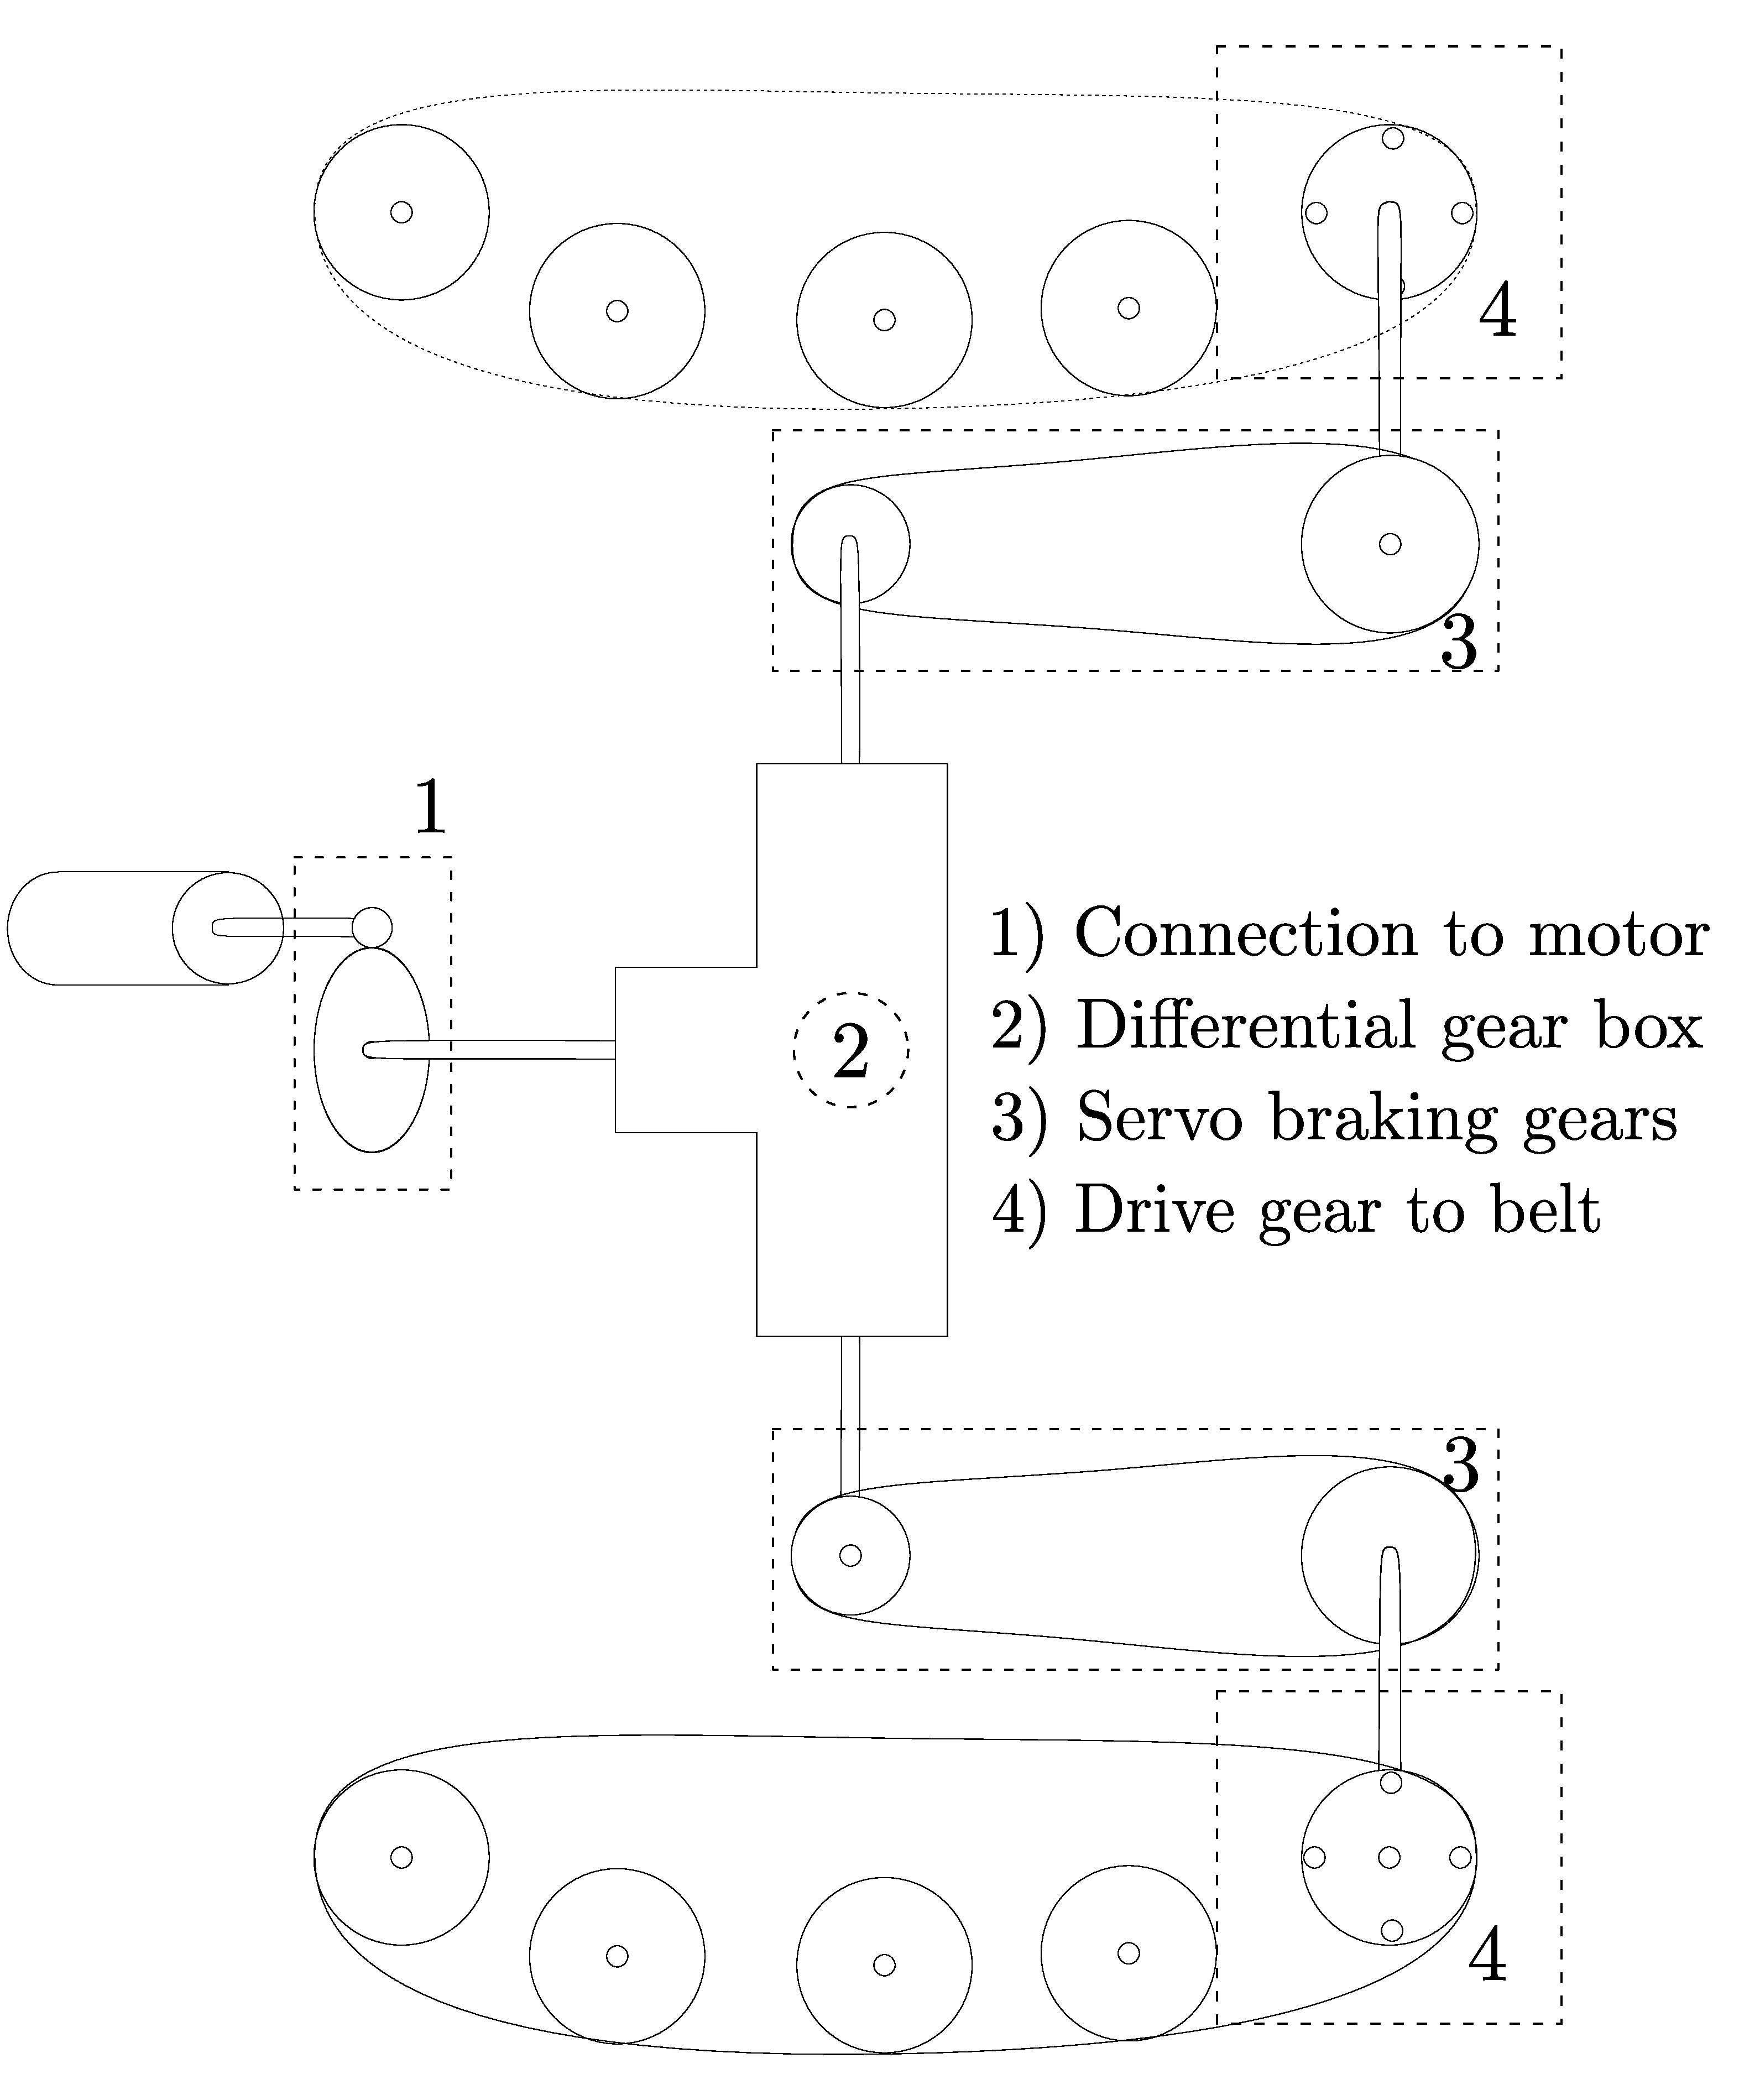
\includegraphics[scale=0.2]{figures/vehicleDescriptionDriveTrain.pdf}
	\caption{Illustration of the drive train of the vehicle.}
	\label{vehicleDescriptionDriveTrain}
\end{figure}

The motor apply a force to the system at the start of the drivetrain(1). The differential gear box(2) is direclty connected to the motor. The servo controls the steering, by applying a breaking force on the breaking gears(3). The rotational power is then transmitted to the other track through the differential gear box(2). The vehicle runs on two belts, that envelop on each side 4 free wheels, plus a gear wheel connected to the drivetrain(4). A Hall sensor is setup on each gear wheel(4), to measure the speed of each belt.\\
The following sections will describe the different parts of the drivetrain seen on \figref {vehicleDescriptionDriveTrain}.\\